\pagenumbering{Roman}
\begin{appendices}
\section{Unterrichtsverlaufspläne}
\label{app:unterrichtsverlaufspläne}

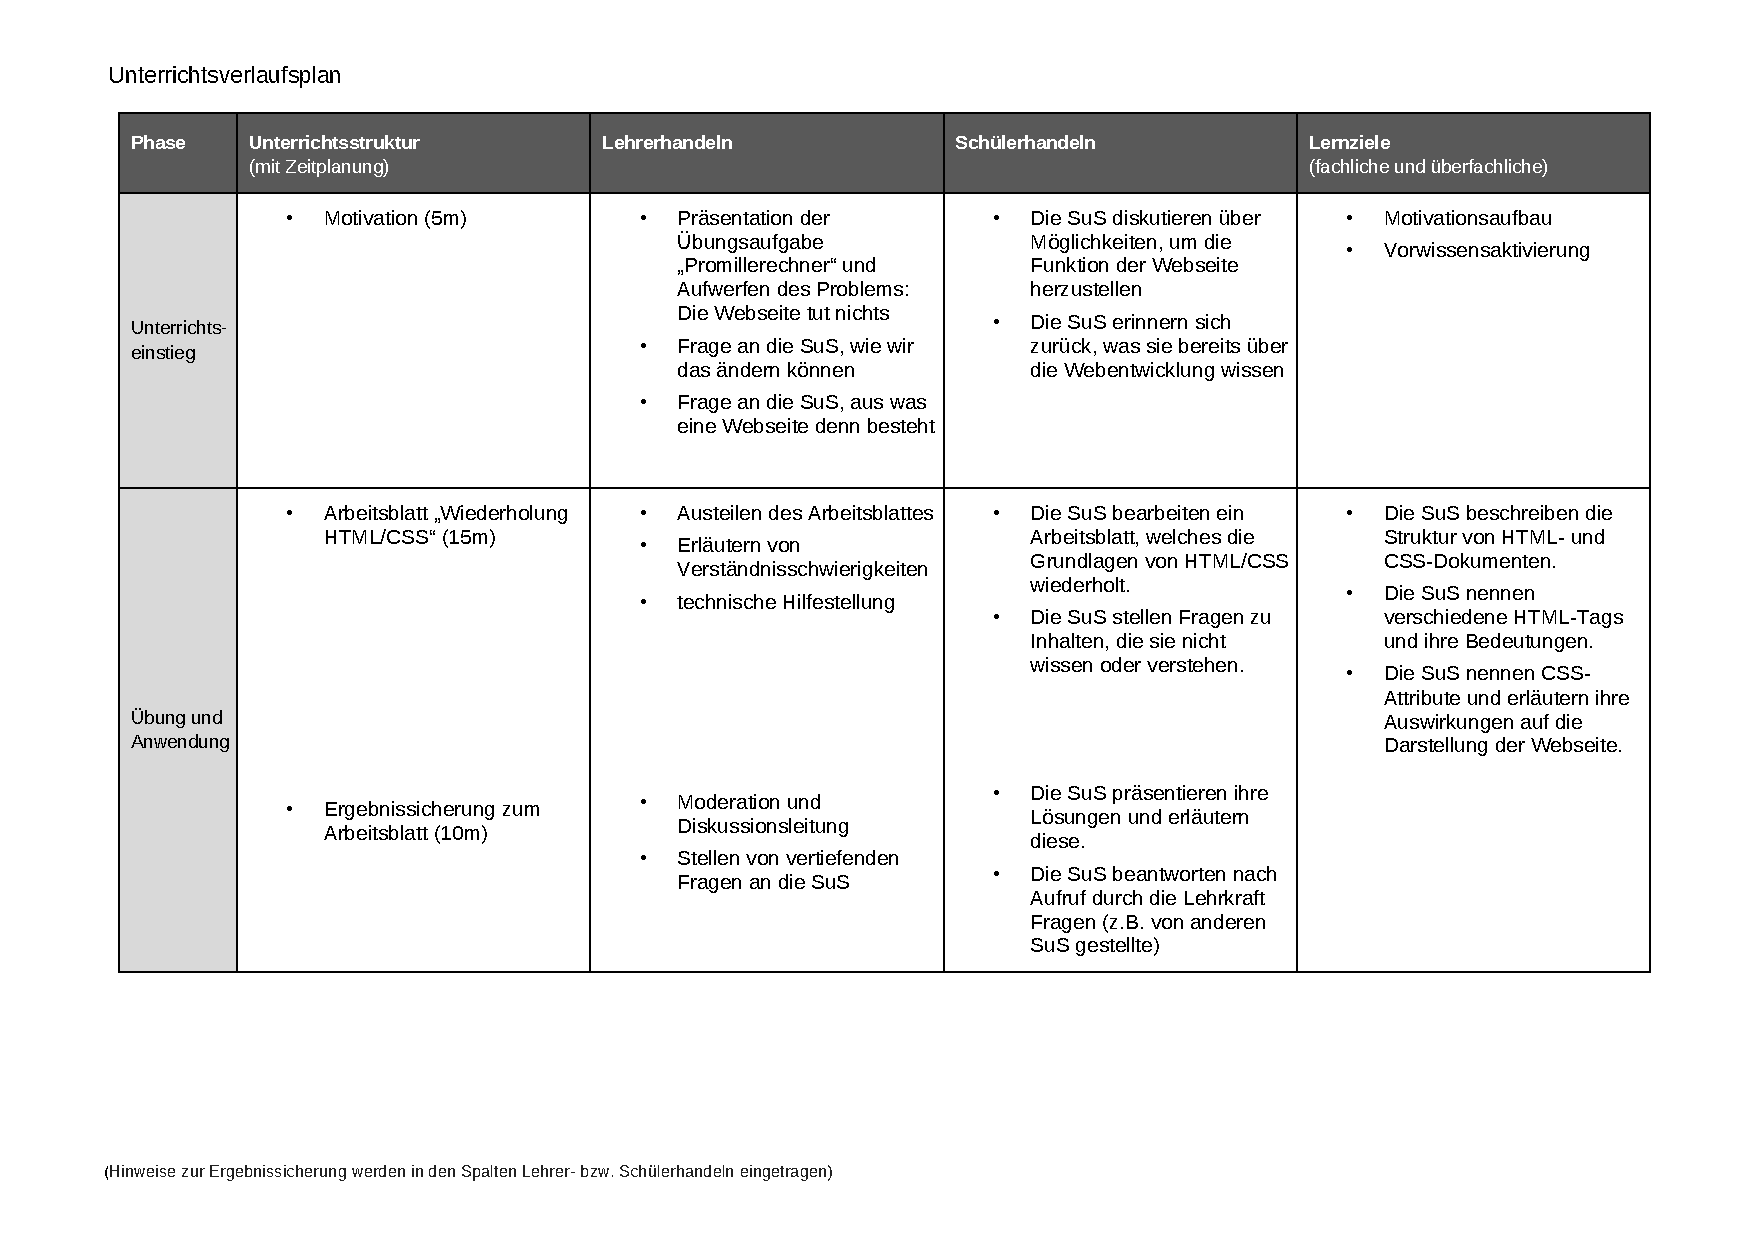
\includepdf[pages={-}, angle=90, scale=0.8, frame, pagecommand={\thispagestyle{plain}},
addtotoc={1, subsection, 2, Unterrichtsverlaufsplan 1, subsec:UVP1}]{appendix/Javascript1/Unterrichtsverlaufsplan.pdf}
\label{pdf:UVP1}
\pagebreak

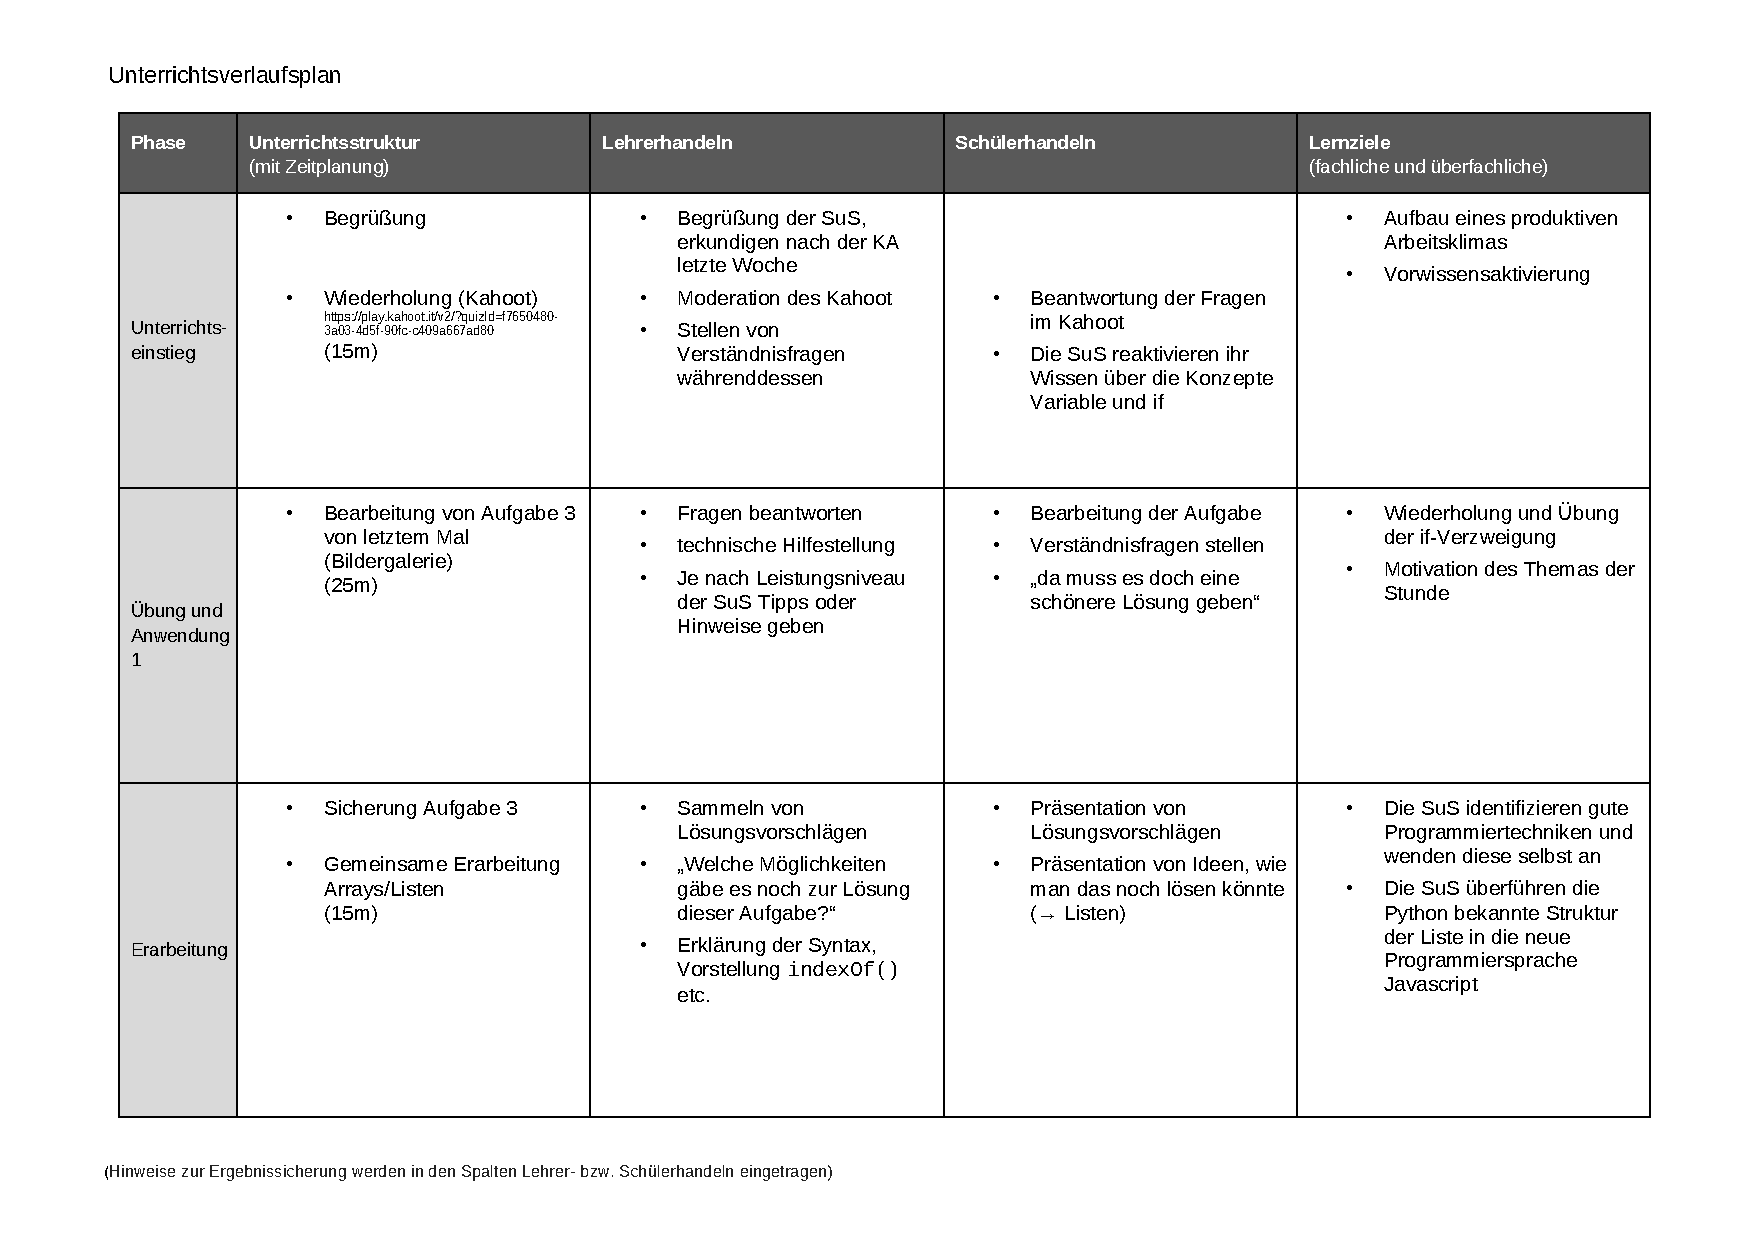
\includepdf[pages={-}, angle=90, scale=0.8, frame, pagecommand={\thispagestyle{plain}},
addtotoc={1, subsection, 2, Unterrichtsverlaufsplan 2, subsec:UVP2}]{appendix/Javascript2/Unterrichtsverlaufsplan.pdf}
\label{pdf:UVP2}
\pagebreak

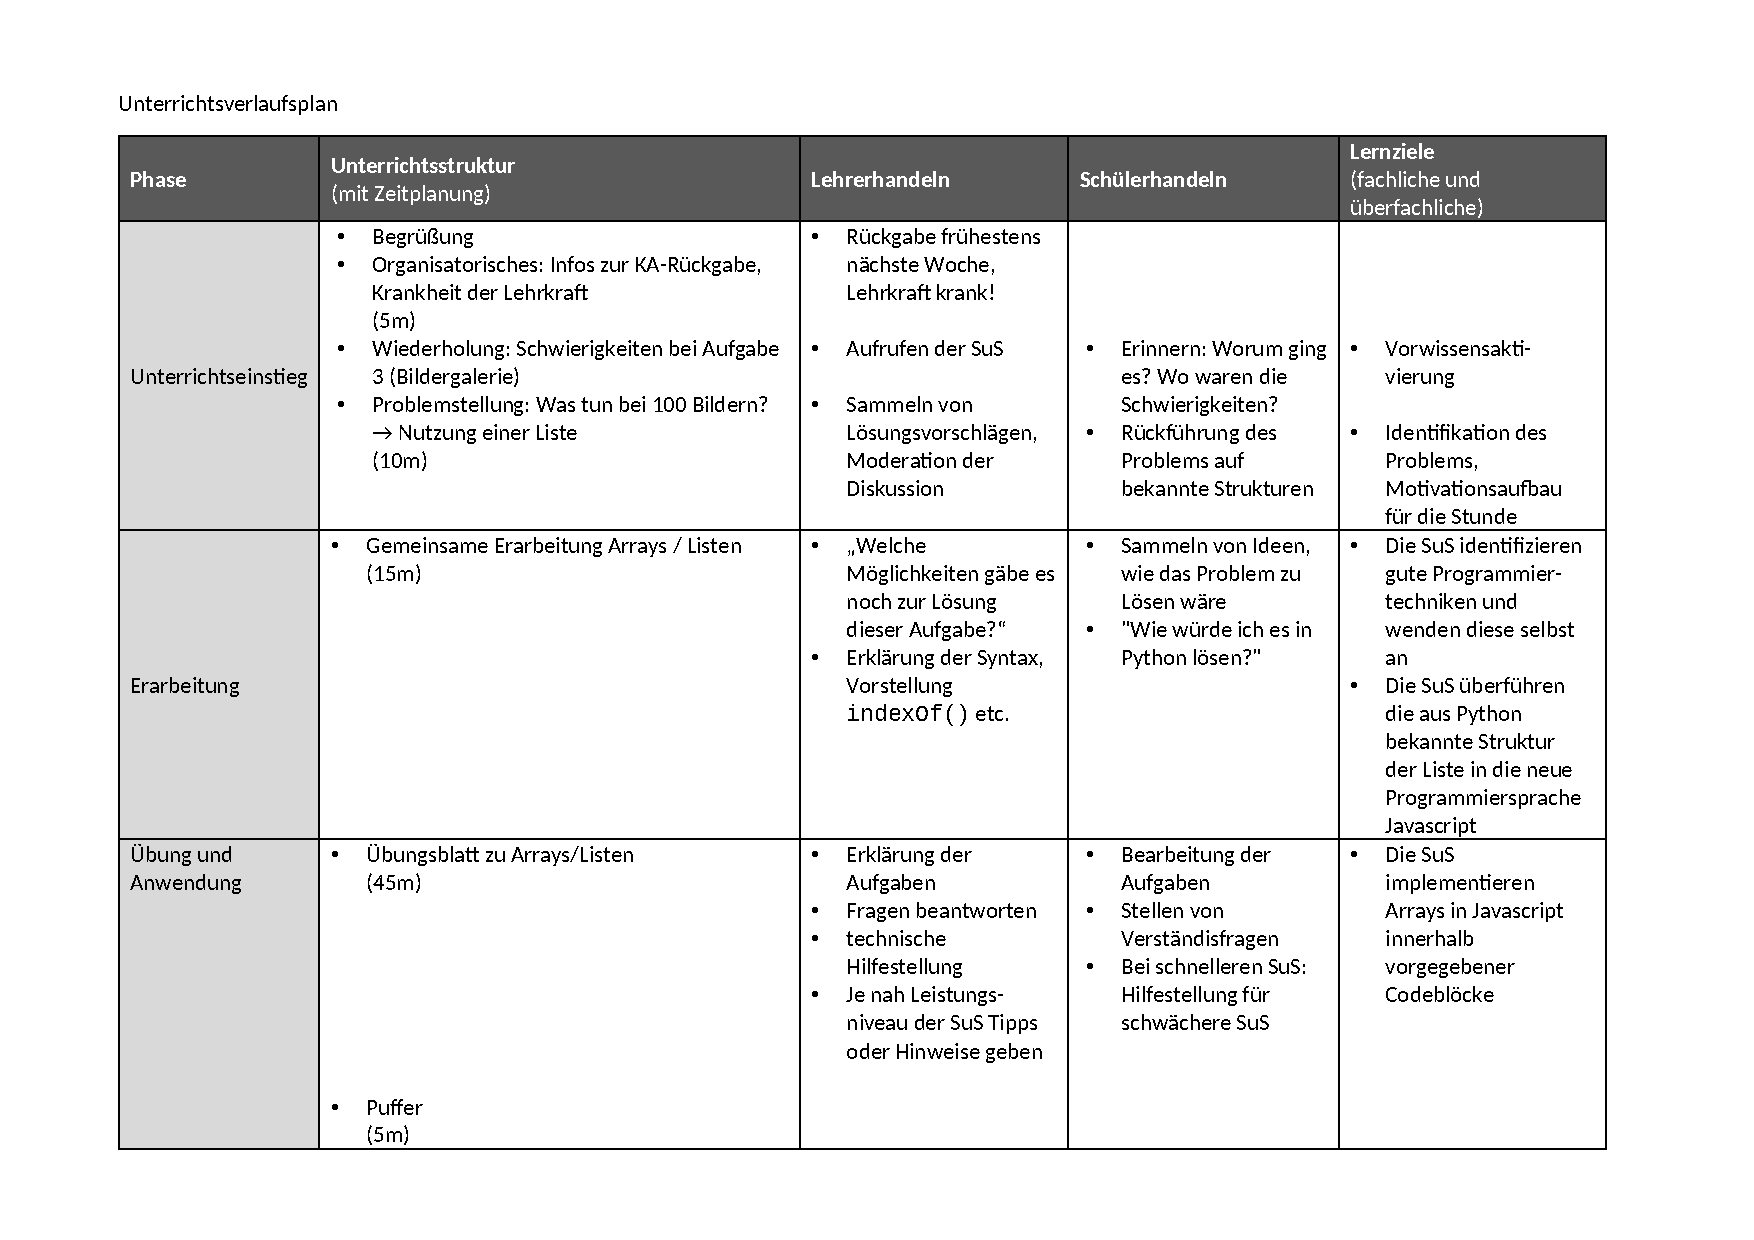
\includepdf[pages={-}, angle=90, scale=0.8, frame,
pagecommand={\thispagestyle{plain}},
addtotoc={1, subsection, 2, Unterrichtsverlaufsplan 3, subsec:UVP3}]{appendix/Javascript3/Unterrichtsverlaufsplan.pdf}
\label{pdf:UVP3}
\pagebreak

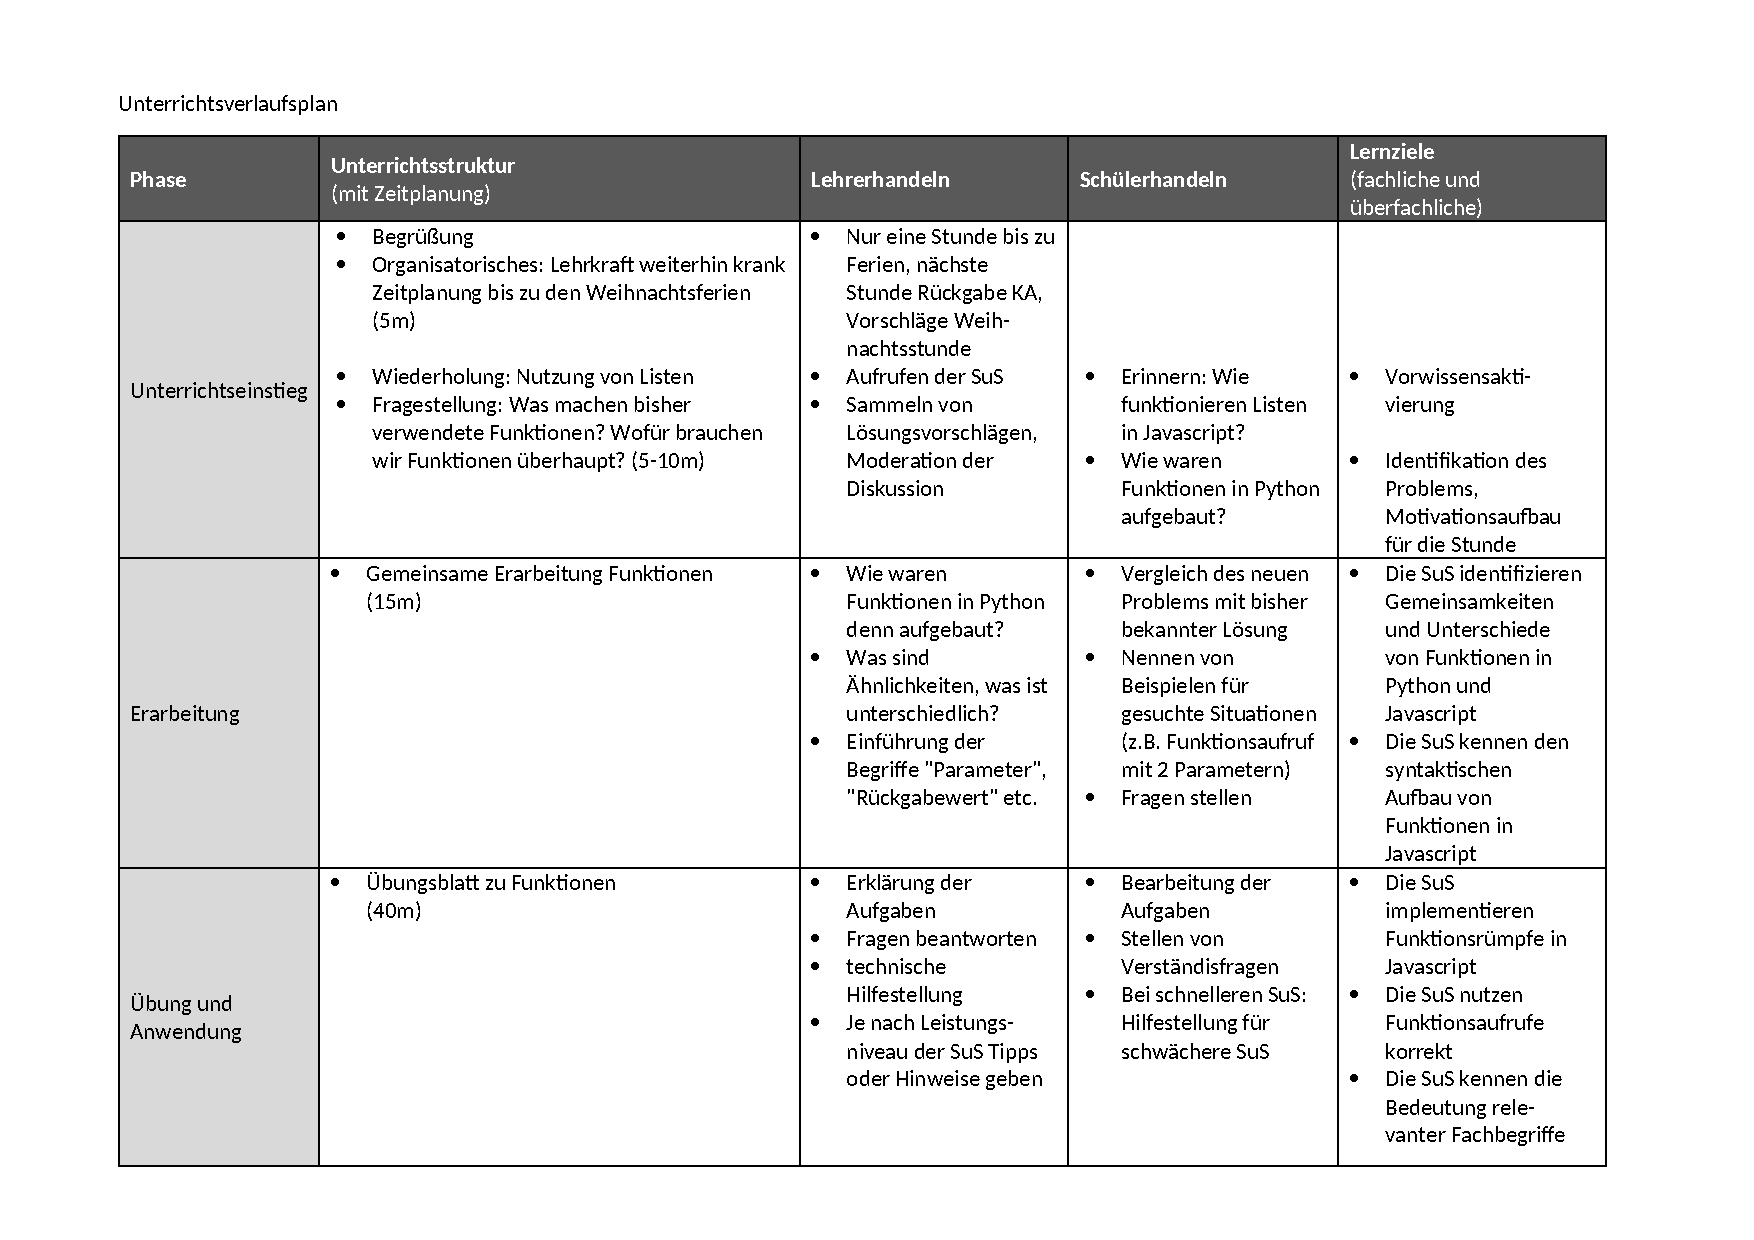
\includepdf[pages={-}, angle=90, scale=0.8, frame,
pagecommand={\thispagestyle{plain}},
addtotoc={1, subsection, 2, Unterrichtsverlaufsplan 4, subsec:UVP4}]{appendix/Javascript4/Unterrichtsverlaufsplan.pdf}
\label{pdf:UVP4}
\pagebreak


\section{Merkblätter}
\label{app:merkblätter}
\pagebreak

\phantomsection
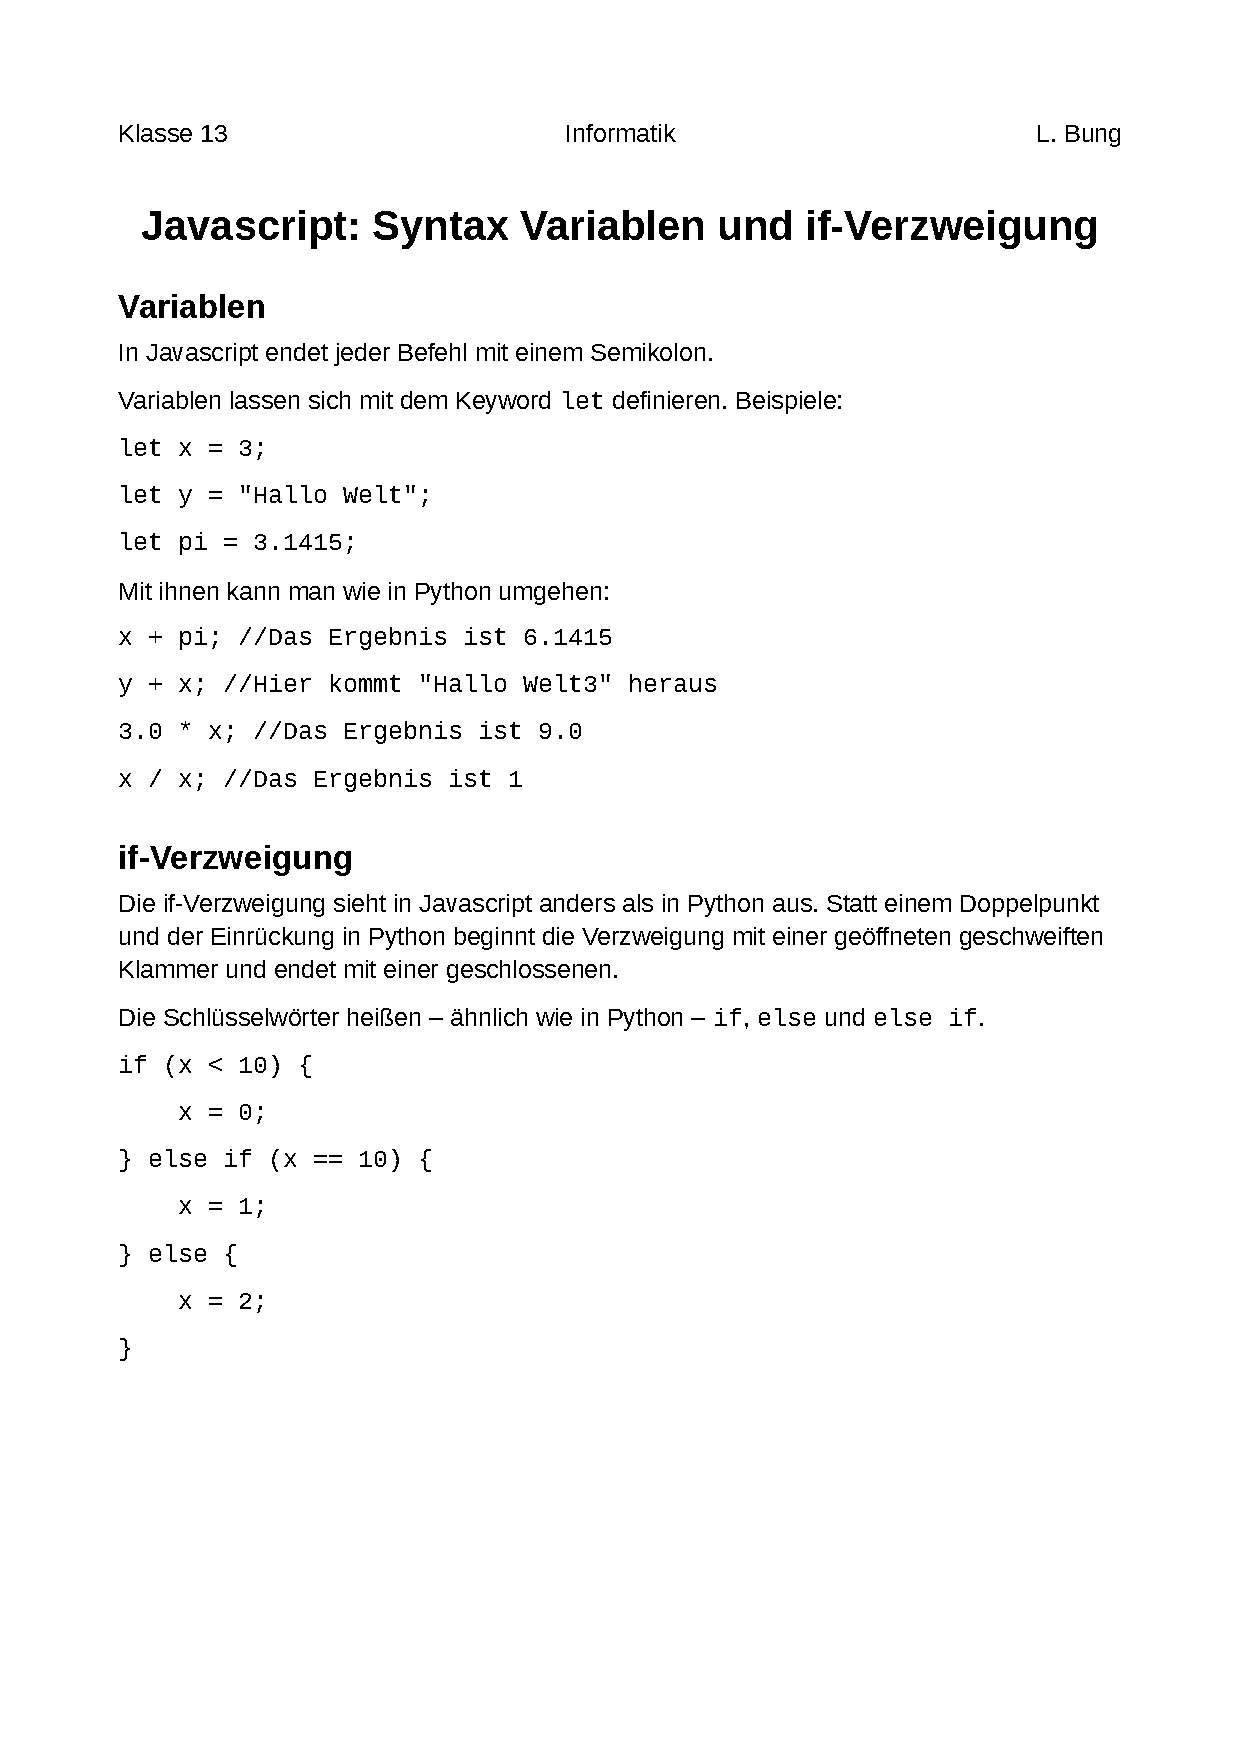
\includepdf[pages={-}, scale=0.8, frame, pagecommand={\thispagestyle{plain}},
addtotoc={1, subsection, 2, Merkblatt Variablen/if, subsec:merkblatt_variablen_if}]{appendix/Javascript1/Merkblatt_Variablen_if.pdf}
\label{pdf:merkblatt_variablen_if}
\pagebreak

\phantomsection
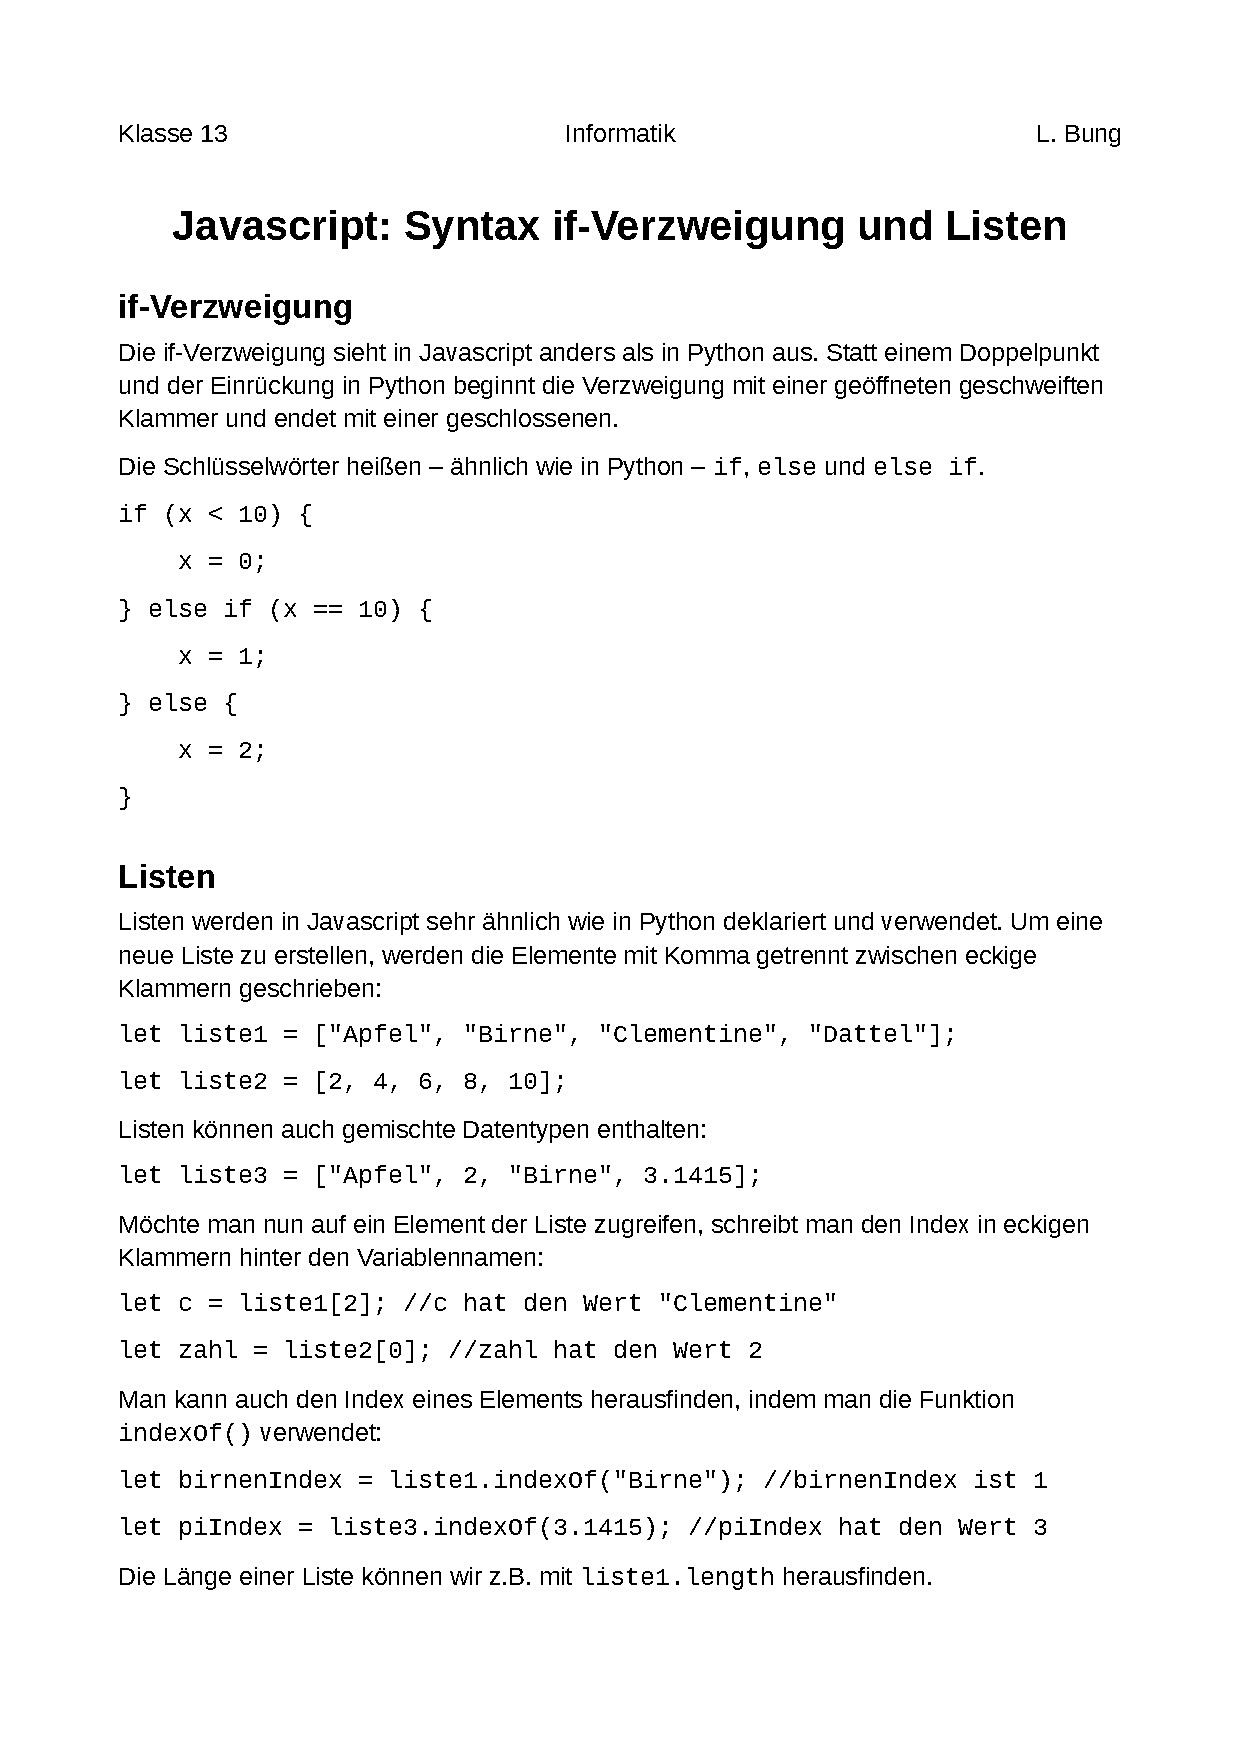
\includepdf[pages={-}, scale=0.8, frame, pagecommand={\thispagestyle{plain}},
addtotoc={1, subsection, 2, Merkblatt if/Listen, subsec:merkblatt_if_listen}]{appendix/Javascript3/Merkblatt_if_Listen.pdf}
\label{pdf:merkblatt_if_listen}
\pagebreak

\phantomsection
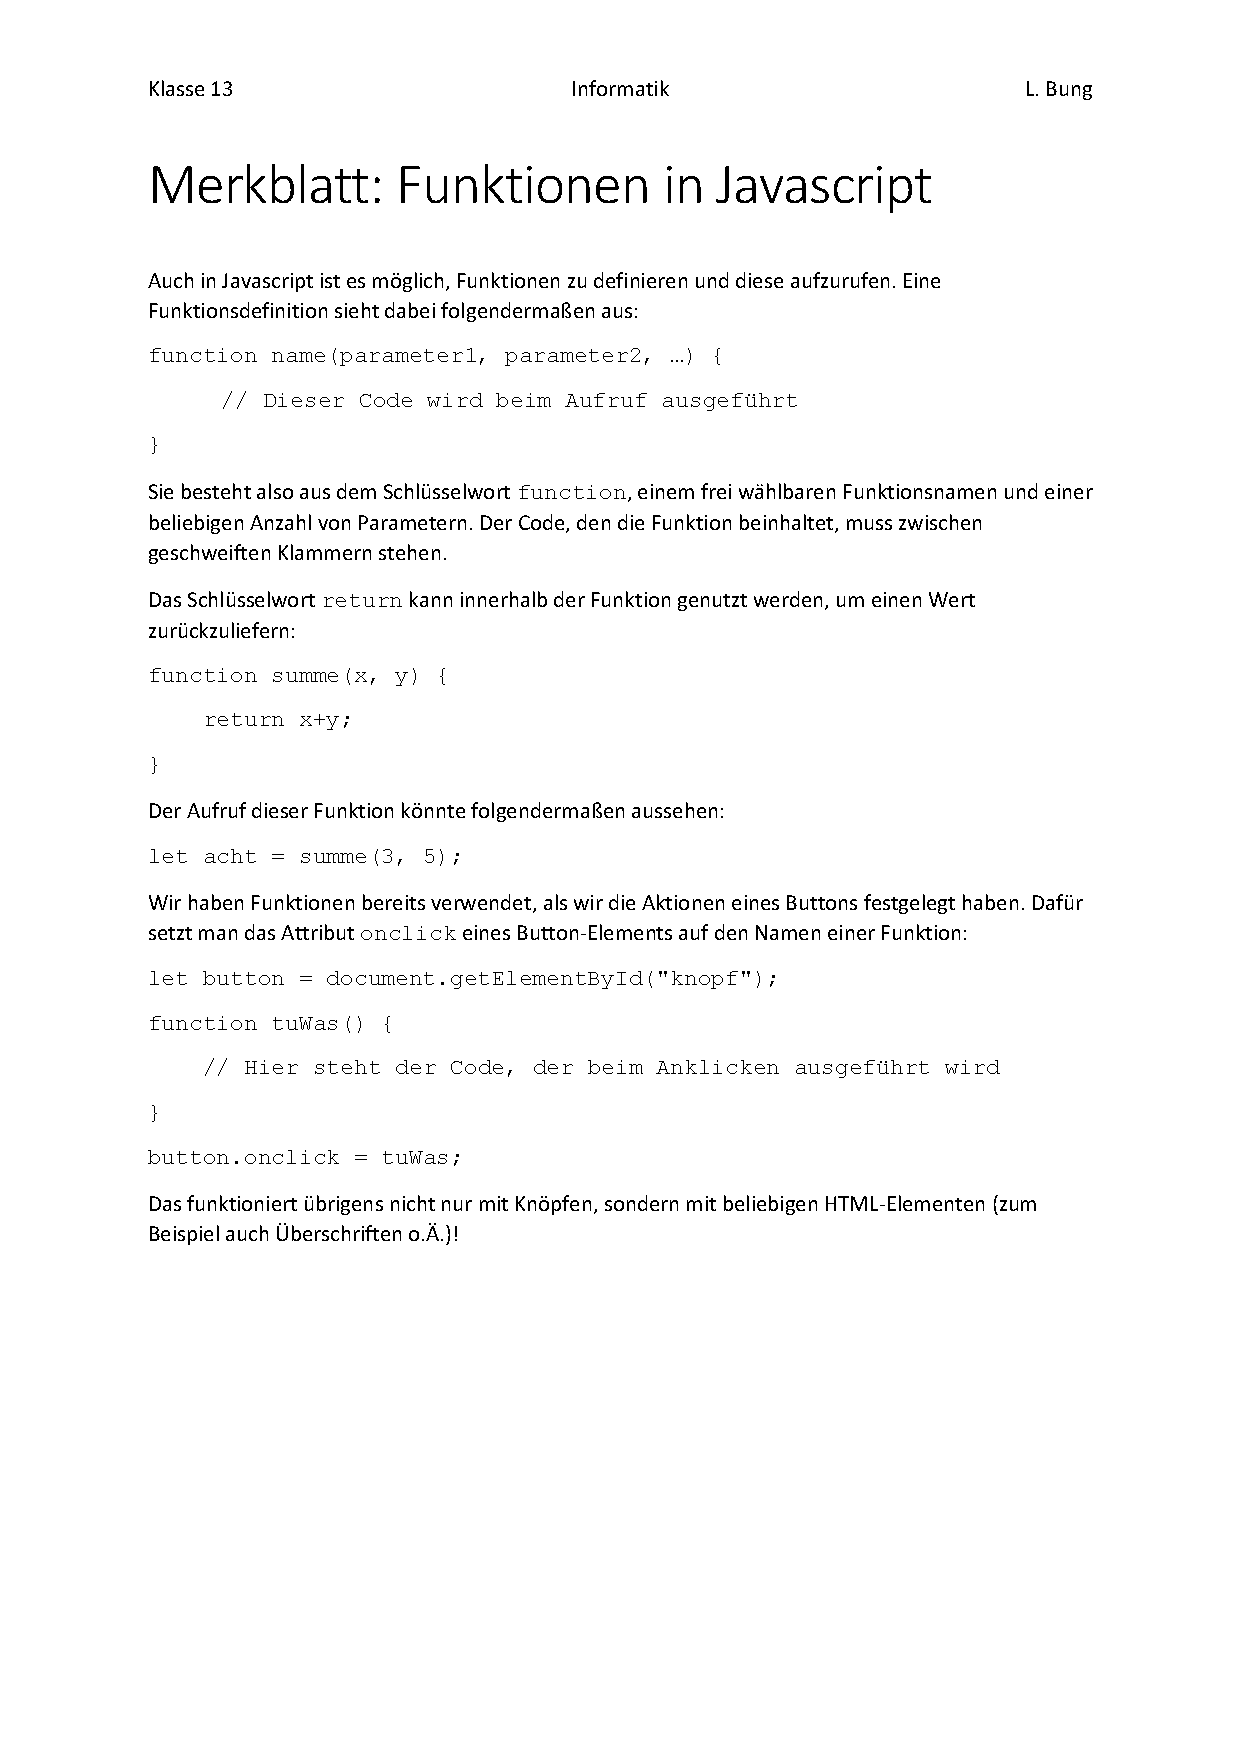
\includepdf[pages={-}, scale=0.8, frame, pagecommand={\thispagestyle{plain}},
addtotoc={1, subsection, 2, Merkblatt Funktionen, subsec:merkblatt_funktionen}]{appendix/Javascript4/Merkblatt_Funktionen.pdf}
\label{pdf:merkblatt_funktionen}


\section{Übungsblätter}
\label{app:übungsblätter}
\pagebreak

\phantomsection
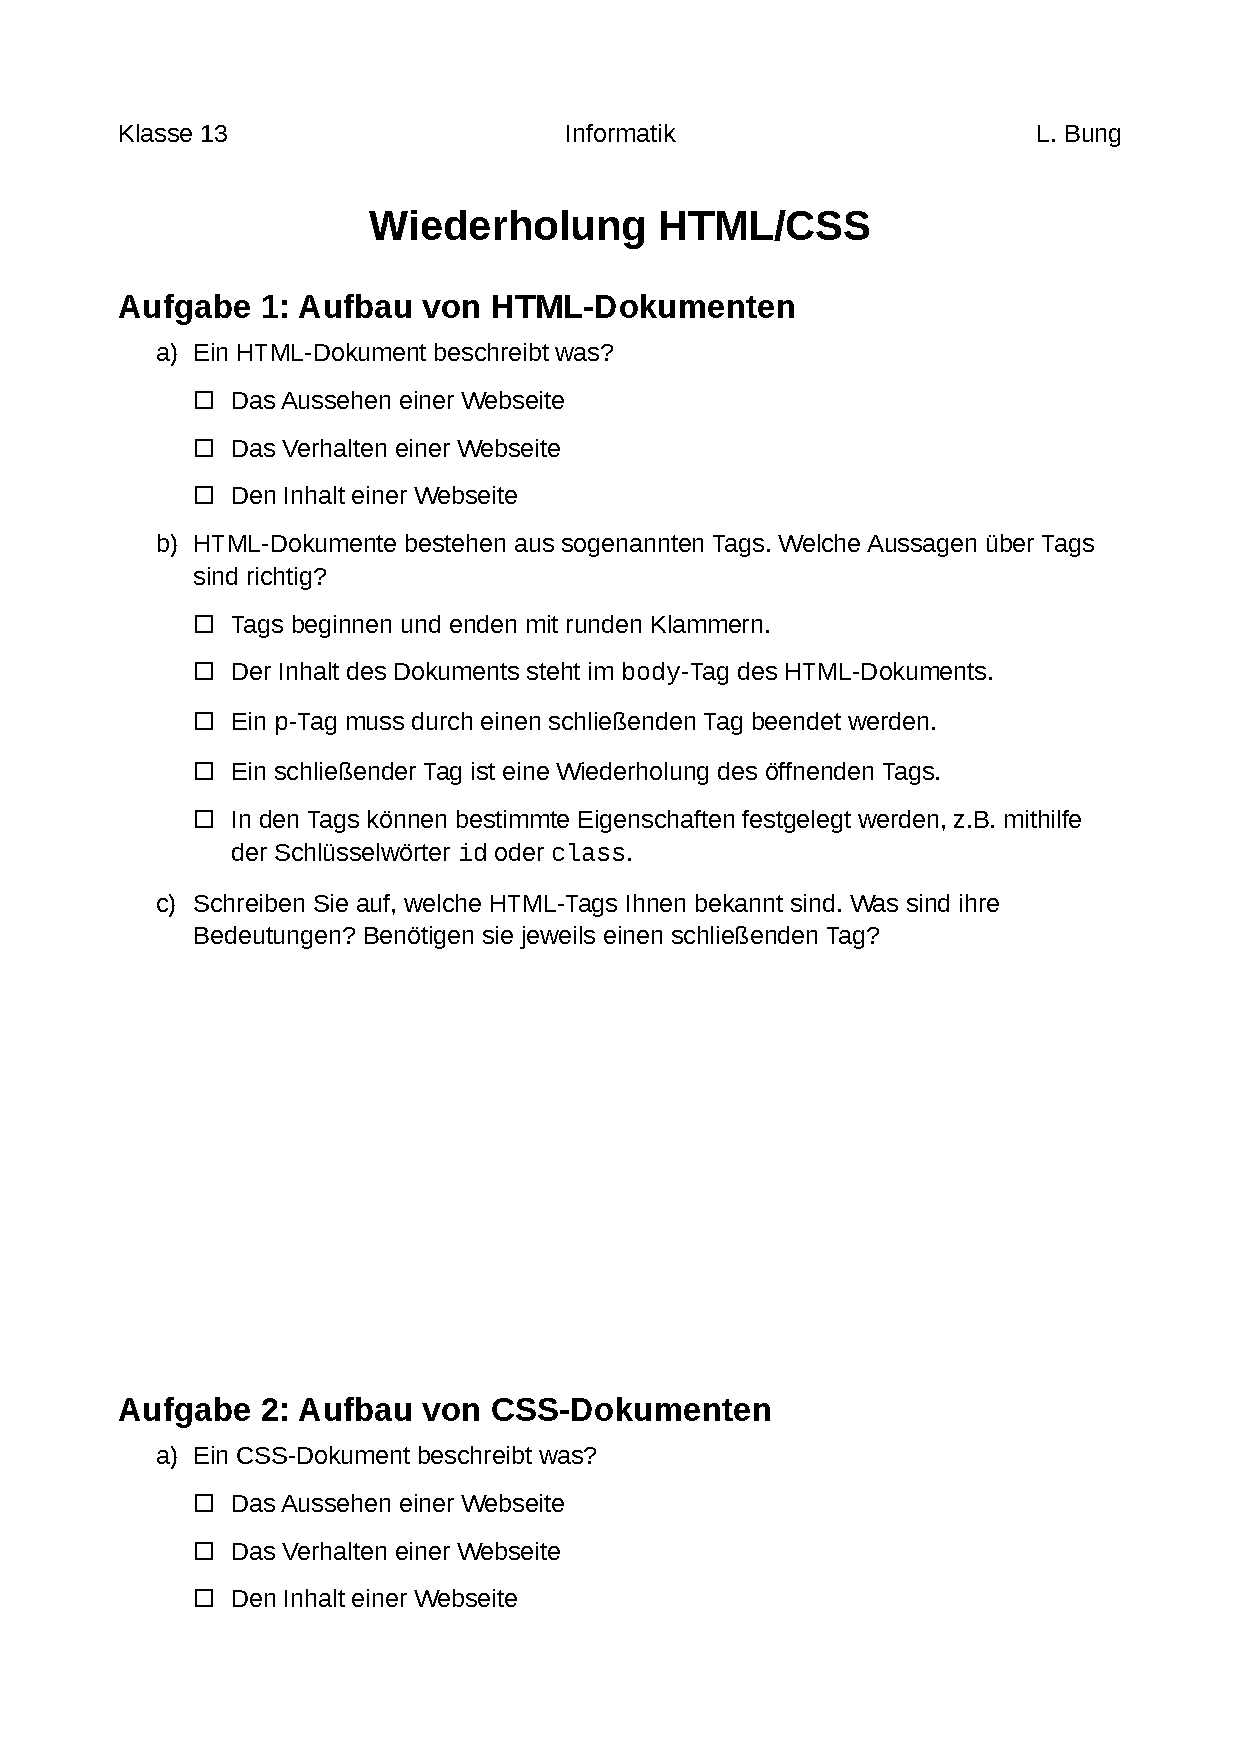
\includepdf[pages={-}, scale=0.8, frame, pagecommand={\thispagestyle{plain}},
addtotoc={1, subsection, 2, Übungsblatt HTML/CSS, subsec:ab_html_css}]{appendix/Javascript1/AB_HTML_CSS.pdf}
\label{pdf:ab_html_css}
\pagebreak

\phantomsection
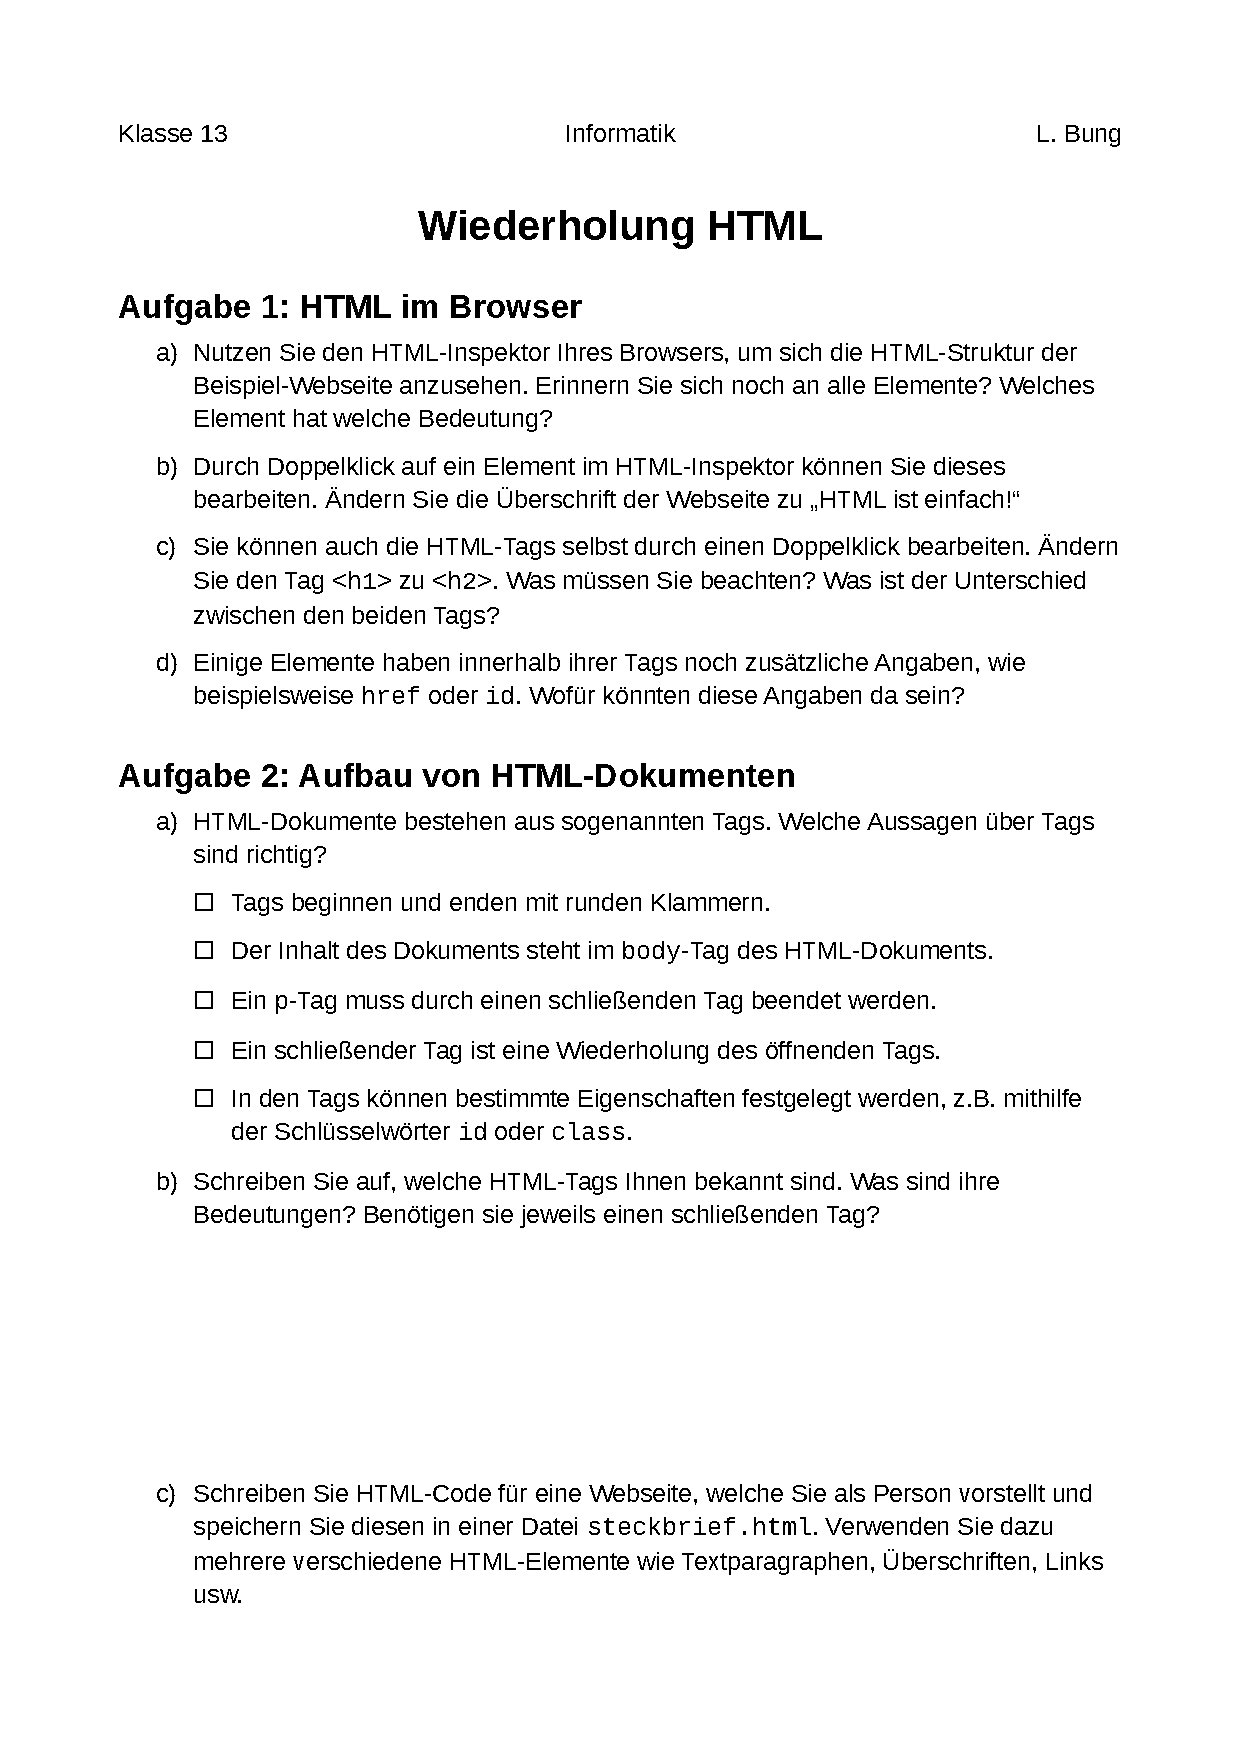
\includepdf[pages={-}, scale=0.8, frame, pagecommand={\thispagestyle{plain}},
addtotoc={1, subsection, 2, Übungsblatt HTML, subsec:ab_html}]{appendix/Javascript1/AB_HTML.pdf}
\label{pdf:ab_html}
\pagebreak

\phantomsection
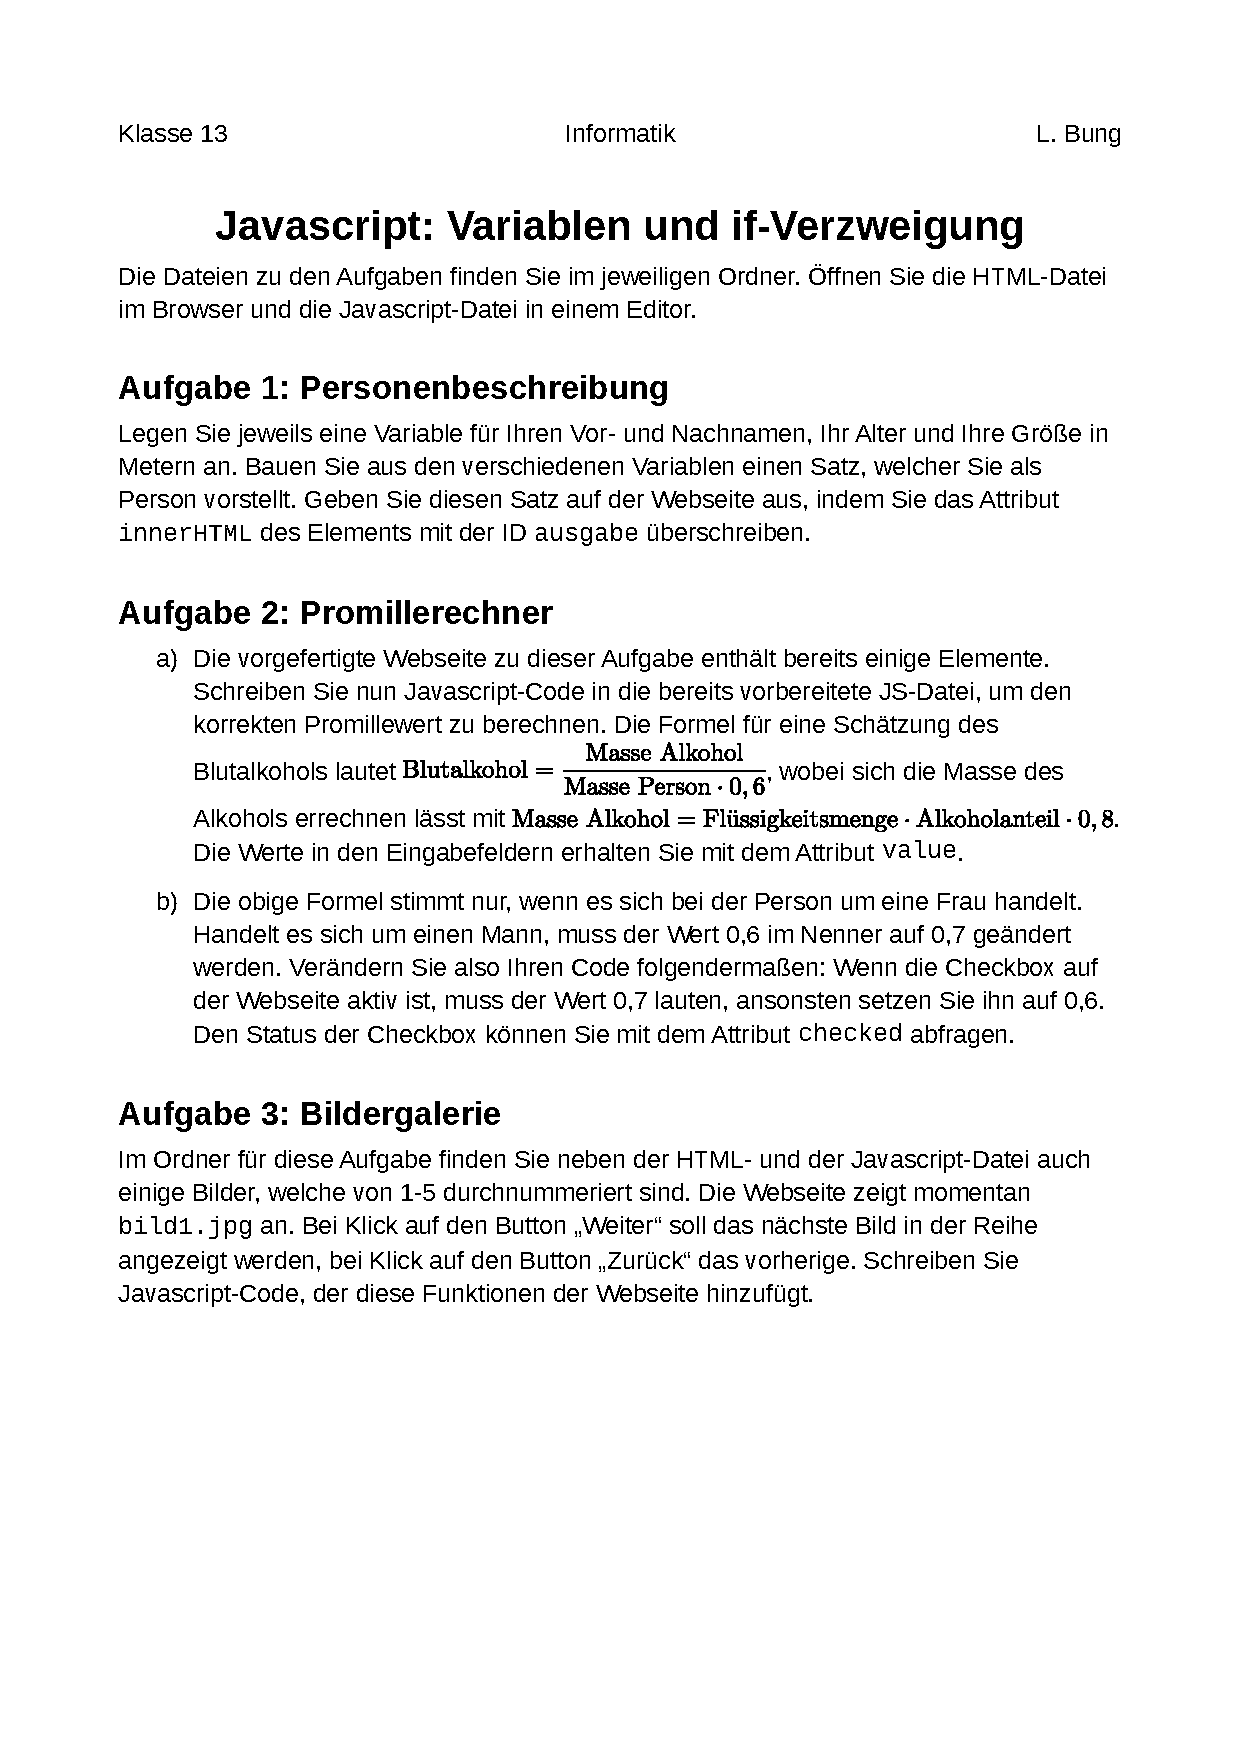
\includepdf[pages={-}, scale=0.8, frame, pagecommand={\thispagestyle{plain}},
addtotoc={1, subsection, 2, Übungsblatt Variablen/if, subsec:ab_variablen_if}]{appendix/Javascript1/AB_Variablen_if.pdf}
\label{pdf:ab_variablen_if}
\pagebreak

\phantomsection
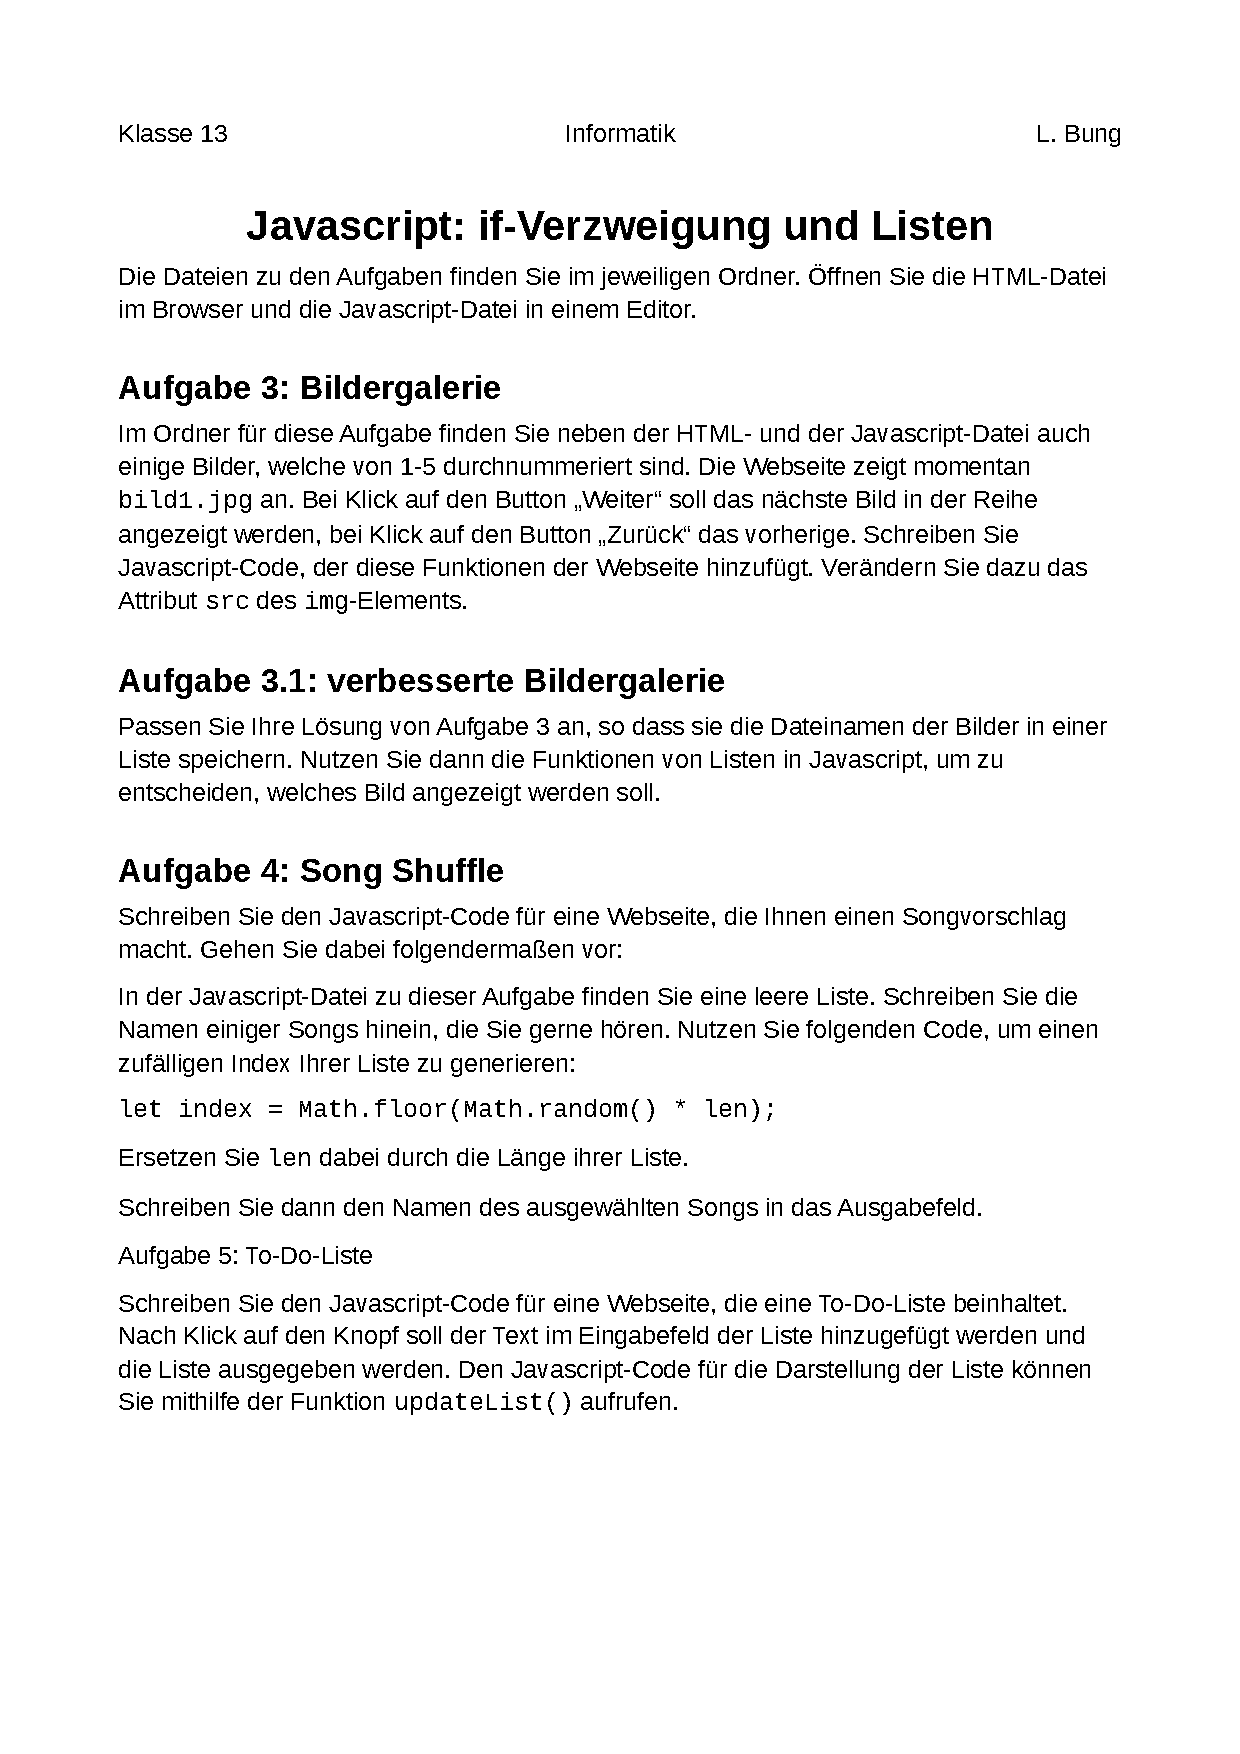
\includepdf[pages={-}, scale=0.8, frame,
pagecommand={\thispagestyle{plain}},
addtotoc={1, subsection, 2, Übungsblatt if/Listen, subsec:ab_if_listen}]{appendix/Javascript3/AB_if_Listen.pdf}
\label{pdf:ab_if_listen}
\pagebreak

\phantomsection

\includepdf[pages={-}, scale=0.8, frame,
pagecommand={\thispagestyle{plain}},
addtotoc={1, subsection, 2, Übungsblatt Funktionen, subsec:ab_funktionen}]{appendix/Javascript4/AB_Funktionen.pdf}
\label{pdf:ab_funktionen}

\section{Codegerüste zu den Übungsaufgaben}
\label{app:codegerüste}

\subsection{Aufgabe 0: Wiederholung HTML}
\label{app:code0}

\lstinputlisting[style=htmlcssjs, label=lst:code0, , caption={Code zu Aufgabe 0: Wiederholung HTML}]{appendix/Aufgaben/Aufgabe0/aufgabe0.html}


\subsection{Aufgabe 1: Personenbeschreibung}
\label{app:code1}

\lstinputlisting[style=htmlcssjs, label=lst:code1-html, caption={HTML-Code zu Aufgabe 1: Personenbeschreibung}]{appendix/Aufgaben/Aufgabe1/aufgabe1.html}

\lstinputlisting[style=htmlcssjs, label=lst:code1-js, caption={Javascript-Codegerüst zu Aufgabe 1: Personenbeschreibung}]{appendix/Aufgaben/Aufgabe1/aufgabe1.js}


\subsection{Aufgabe 2: Promillerechner}
\label{app:code2}

\lstinputlisting[style=htmlcssjs, label=lst:code2-html, caption={HTML-Code zu Aufgabe 2: Promillerechner}]{appendix/Aufgaben/Aufgabe2/aufgabe2.html}

\lstinputlisting[style=htmlcssjs, label=lst:code2-js, caption={Javascript-Codegerüst zu Aufgabe 2: Promillerechner}]{appendix/Aufgaben/Aufgabe2/aufgabe2.js}


\subsection{Aufgabe 3: Bildergalerie}
\label{app:code3}

\lstinputlisting[style=htmlcssjs, label=lst:code3-html, caption={HTML-Code zu Aufgabe 3: Bildergalerie}]{appendix/Aufgaben/Aufgabe3/aufgabe3.html}

\lstinputlisting[style=htmlcssjs, label=lst:code3-js, caption={Javascript-Codegerüst zu Aufgabe 3: Bildergalerie}]{appendix/Aufgaben/Aufgabe3/aufgabe3.js}


\subsection{Aufgabe 4: Song Shuffle}
\label{app:code4}

\lstinputlisting[style=htmlcssjs, label=lst:code4-html, caption={HTML-Code zu Aufgabe 4: Song Shuffle}]{appendix/Aufgaben/Aufgabe4/aufgabe4.html}

\lstinputlisting[style=htmlcssjs, label=lst:code4-js, caption={Javascript-Codegerüst zu Aufgabe 4: Song Shuffle}]{appendix/Aufgaben/Aufgabe4/aufgabe4.js}


\subsection{Aufgabe 5: To-Do-Liste}
\label{app:code5}

\lstinputlisting[style=htmlcssjs, label=lst:code5-html, caption={HTML-Code zu Aufgabe 5: To-Do-Liste}]{appendix/Aufgaben/Aufgabe5/aufgabe5.html}

\lstinputlisting[style=htmlcssjs, label=lst:code5-js, caption={Javascript-Codegerüst zu Aufgabe 5: To-Do-Liste}]{appendix/Aufgaben/Aufgabe5/aufgabe5.js}


\subsection{Aufgabe 6: Taschenrechner 1}
\label{app:code6}

\lstinputlisting[style=htmlcssjs, label=lst:code6-html, caption={HTML-Code zu Aufgabe 6: Taschenrechner 1}]{appendix/Aufgaben/Aufgabe6/aufgabe6.html}


\subsection{Aufgabe 7: Klickzähler}
\label{app:code7}

\lstinputlisting[style=htmlcssjs, label=lst:code7-html, caption={HTML-Code zu Aufgabe 7: Klickzähler}]{appendix/Aufgaben/Aufgabe7/aufgabe7.html}


\subsection{Aufgabe 8: Taschenrechner 2}
\label{app:code8}

\lstinputlisting[style=htmlcssjs, label=lst:code8-html, caption={HTML-Code zu Aufgabe 8: Taschenrechner 2}]{appendix/Aufgaben/Aufgabe8/aufgabe8.html}


\section{Ausdrucke der ersten Seiten der Onlineliteratur}
\pagebreak

\phantomsection

\includepdf[pages={1}, scale=0.7, frame,
pagecommand={\thispagestyle{plain} \cite{bildungsplan-tg-informatik}}]{onlinequellen/Bildungsplan_Beruflich_TG_Informatik.pdf}
\pagebreak

\phantomsection
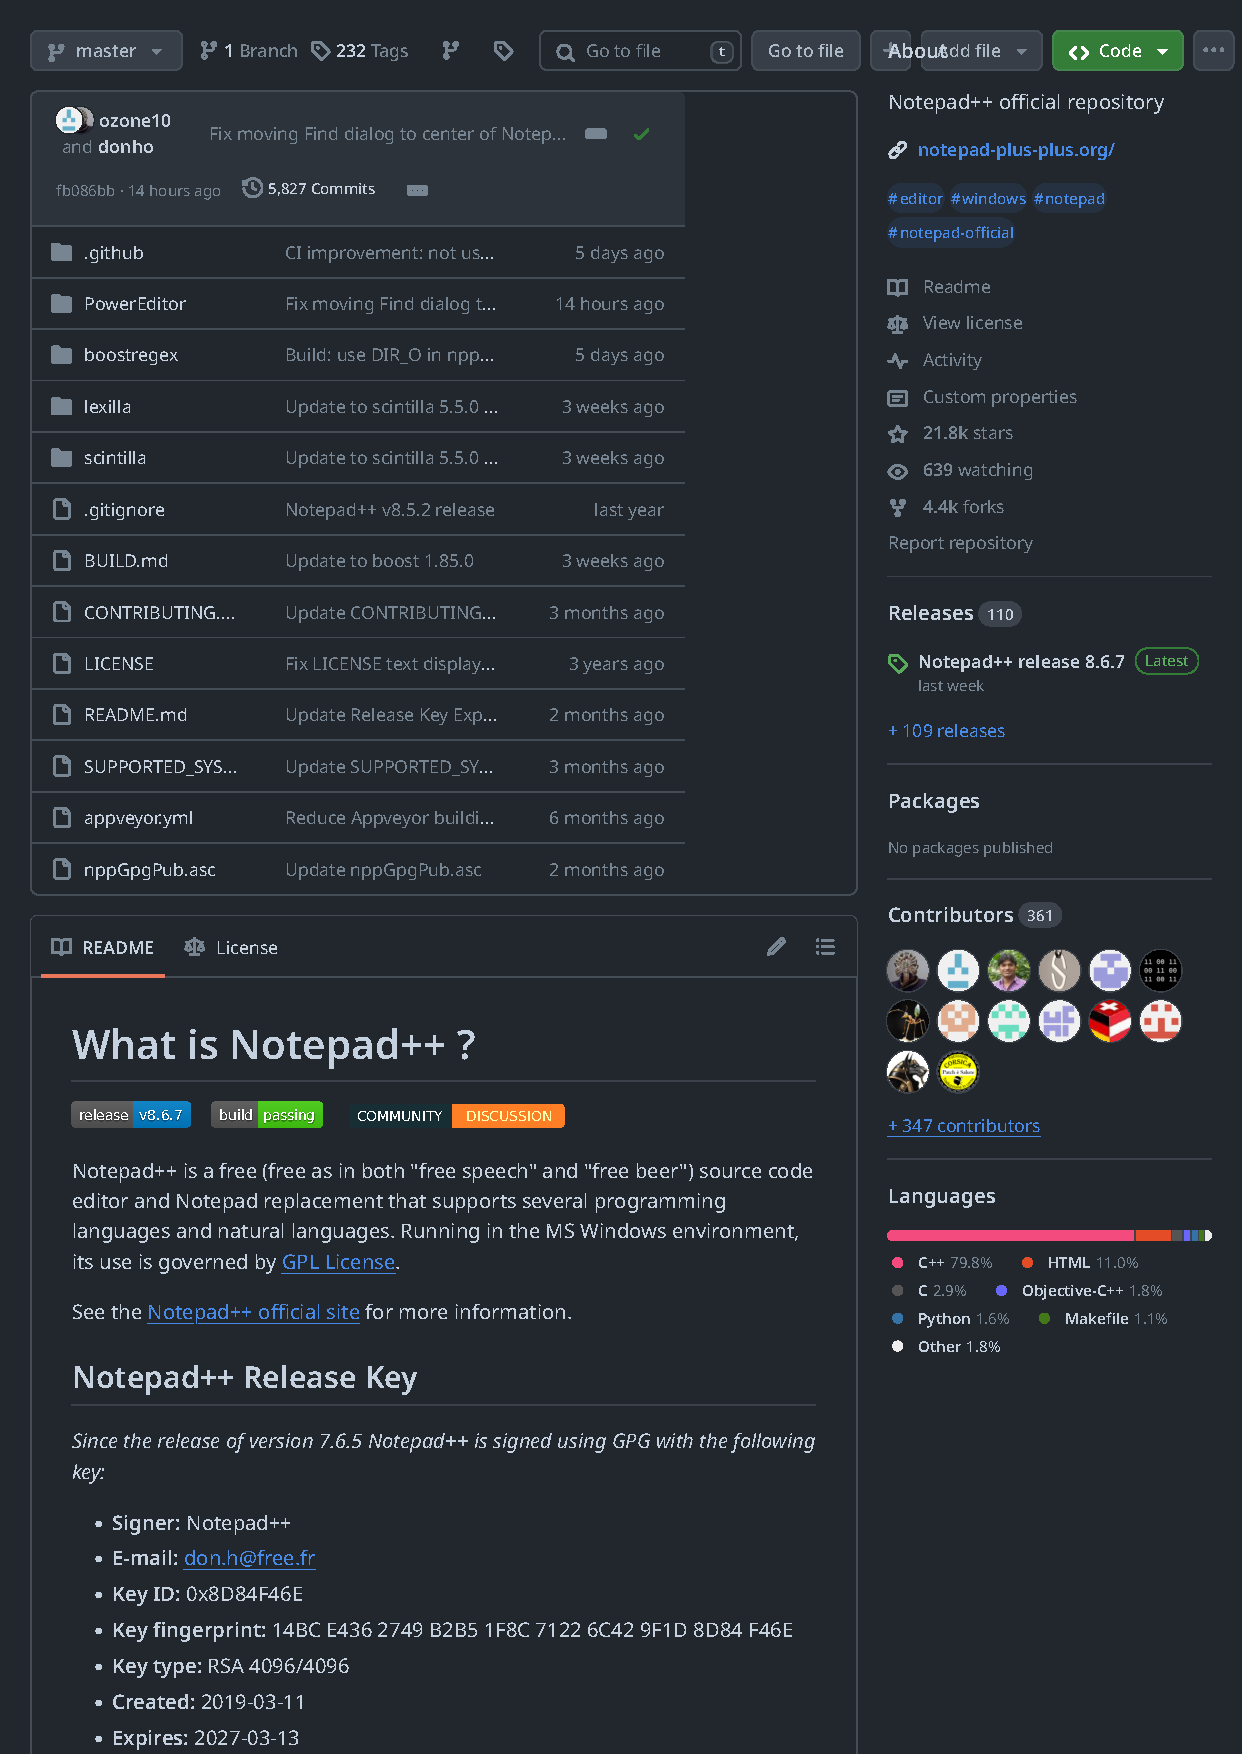
\includepdf[pages={1}, scale=0.7, frame,
pagecommand={\thispagestyle{plain} \cite{ho2021notepad++}}]{onlinequellen/notepad++_github.pdf}
\pagebreak

\phantomsection
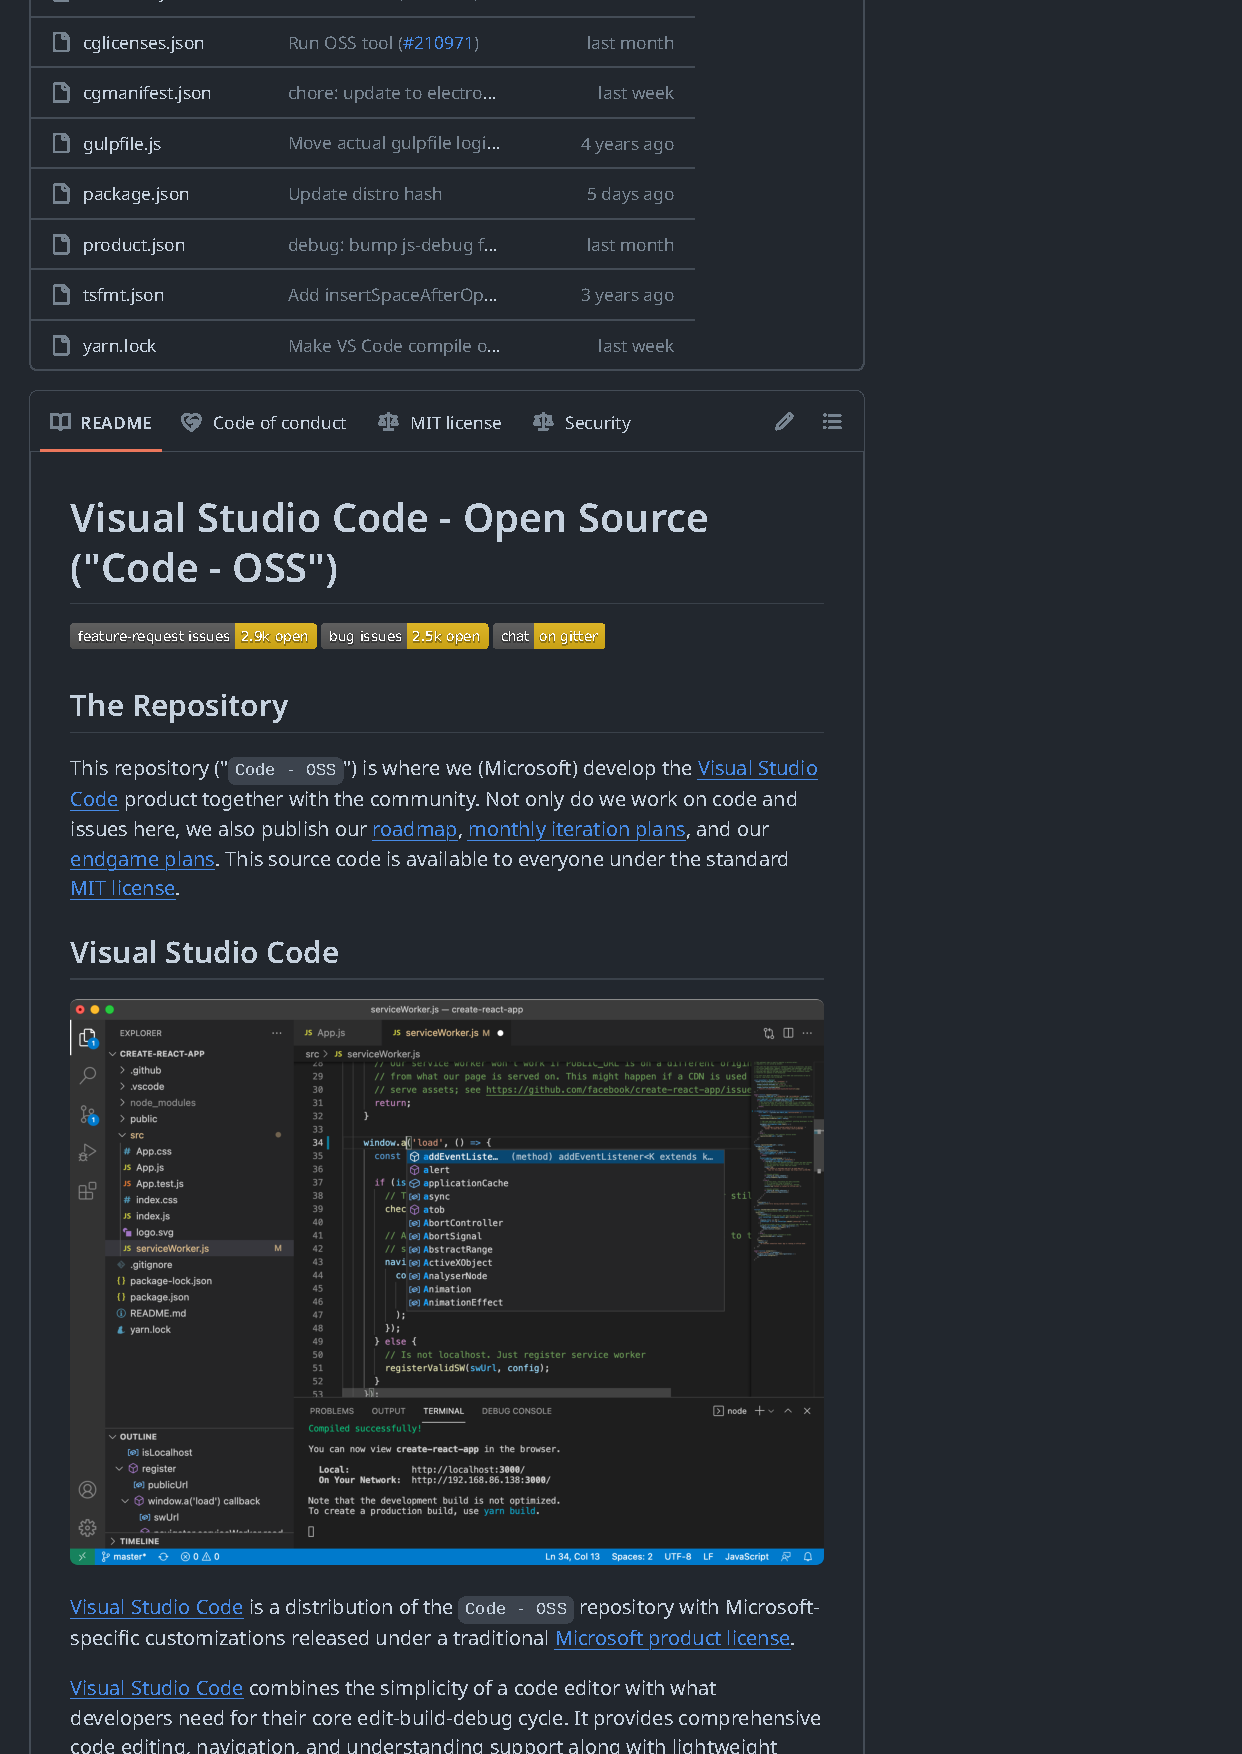
\includepdf[pages={1}, scale=0.7, frame,
pagecommand={\thispagestyle{plain} \cite{microsoft2024vscode}}]{onlinequellen/vscode_github.pdf}
\end{appendices}